% ============================================================
% 数电实验报告
% ============================================================

\documentclass[12pt]{ctexart}

% --- 宏包 ---
\usepackage{graphicx}
\usepackage{amsmath}
\usepackage{listings}
\usepackage{float}
\usepackage{booktabs}
\usepackage{siunitx}
\usepackage{fancyhdr}
\usepackage{caption}
\usepackage{subcaption}
\usepackage{hyperref}
\usepackage{makecell}
\usepackage{enumitem}

\sisetup{per-mode=symbol}

\graphicspath{{./figures/}{../figures/}}

\usepackage[left=2.5cm, right=2.5cm, top=2.5cm, bottom=2.5cm]{geometry}

\setlength{\jot}{6pt}
\setlength{\headheight}{15pt}
\linespread{1.5}
\setlist{nosep}

% --- 页眉页脚 ---
\pagestyle{fancy}
\fancyhead[C]{数字电子技术实验}
\fancyfoot[C]{\thepage}

\begin{document}

% ==================== 封面 ====================
\thispagestyle{empty}

\begin{figure}[t]
    \centering
    
\includegraphics[width=13cm]{logo1.png}
\end{figure}

\vspace*{\fill}
    \begin{center}
        \Huge\textbf{数字电子技术基础}

        \vspace{0.3cm}
        \Huge\textbf{实验报告}

        \vspace{1cm}
        \LARGE\textbf{实验三：时序电路设计与数码管显示}
    \end{center}
\vspace*{\fill}

\begin{table}[H]
    \centering
    \large
    \begin{tabular}{ll}
    \toprule
    \textbf{课程:} & 数字电子技术实验 \\
    \textbf{组员1:} & 郭浩然 2024303980 \\
    \textbf{组员2:} & 庞铭洋 2024302539 \\
    \textbf{组号:} & 15 \\
    \textbf{时间:} & \today \\
    \bottomrule
    \end{tabular}
\end{table}

\newpage

% ==================== 正文 ====================

\section{实验目的}

\begin{enumerate}
    \item 掌握时序逻辑电路的基本设计方法，理解计数、译码和显示控制之间的关系。
    \item 学习七段数码管显示电路的设计方法，掌握数字编码到段选信号的转换过程。
    \item 掌握利用 Quartus II 进行原理图设计和波形仿真的基本流程。
    \item 能够根据给定数字序列设计显示控制逻辑，并通过仿真波形验证功能正确性。
\end{enumerate}

\section{实验要求}

根据实验要求图片，本实验内容如下：

\begin{enumerate}
    \item 参照参考内容中数码管显示控制电路设计方法，用计数器、七段译码器和若干门电路，用原理图输入方法，在一个 7 段数码管上显示序列：学号（组员 A 学号后 8 位，组员 B 学号后 4 位）。
    \item 用计数器 7490 完成要求 1 中学号循环显示的计数，并显示在数码管中（用一个数码管显示轮次即可）。
\end{enumerate}

要求提交或展示的内容包括：原理图、波形仿真，并下载到 FPGA 验证。

根据补充说明，12 位显示数据选取为\texttt{243025393980}

其中前八位为组员学号后八位 \texttt{24302539}，后四位为另一组员学号后四位 \texttt{3980}。

\section{实验设备}

\begin{itemize}
    \item Quartus II 开发软件
    \item DE0 开发板（FPGA 型号：Cyclone V 5CEBA4F23C7）
    \item USB-Blaster 下载线及计算机
    \item 七段数码管显示模块及相关输入、输出引脚
\end{itemize}

\section{实验原理}

\subsection{时序显示控制}

时序逻辑电路的输出不仅与当前输入有关，还与电路当前状态有关。本实验中，显示控制电路需要依次输出 12 位数字，因此可使用计数器产生当前显示位置，再由组合逻辑根据计数状态选择对应数字。计数状态循环变化时，显示内容也随之按预定序列循环输出。

若计数器当前状态记为 $Q$，待显示数字记为 $D$，则显示控制可表示为
\[
    D = f(Q).
\]
其中 $f(Q)$ 按照实验要求依次给出 \texttt{2,4,3,0,2,5,3,9,3,9,8,0}。当计数器完成 12 个状态后回到初始状态，即可实现 12 位数字的循环显示。

\subsection{七段数码管译码}

七段数码管由 $a,b,c,d,e,f,g$ 七个发光段组成。不同数字对应不同段选组合，译码电路根据输入的 BCD 码产生相应段选信号。以共阴极、段选高电平有效为例，常用数字与七段码关系如表~\ref{tab:segment_code} 所示。

\begin{table}[H]
    \centering
    \caption{十进制数字与七段显示关系}
    \label{tab:segment_code}
    \begin{tabular}{c c c}
        \toprule
        \textbf{十进制数字} & \textbf{BCD 码} & \textbf{点亮段} \\
        \midrule
        0 & 0000 & $a,b,c,d,e,f$ \\
        1 & 0001 & $b,c$ \\
        2 & 0010 & $a,b,d,e,g$ \\
        3 & 0011 & $a,b,c,d,g$ \\
        4 & 0100 & $b,c,f,g$ \\
        5 & 0101 & $a,c,d,f,g$ \\
        6 & 0110 & $a,c,d,e,f,g$ \\
        7 & 0111 & $a,b,c$ \\
        8 & 1000 & $a,b,c,d,e,f,g$ \\
        9 & 1001 & $a,b,c,d,f,g$ \\
        \bottomrule
    \end{tabular}
\end{table}

实际实验中若数码管为低电平有效，只需在输出端对段选信号取反。通过计数器、数据选择逻辑和七段译码逻辑的配合，即可将给定数字序列转换为数码管上可观察的显示结果。

\section{实验内容}

\subsection{新建工程}

打开 Quartus II，选择 \textbf{File $\rightarrow$ New Project Wizard} 新建实验三工程。工程目录选择实验三文件夹，顶层实体名与原理图文件名保持一致。器件选择 DE0 开发板对应的 Cyclone V \texttt{5CEBA4F23C7}。工程建立完成后，选择 \textbf{File $\rightarrow$ New $\rightarrow$ Block Diagram/Schematic File} 新建原理图文件，并保存为顶层设计文件。

\subsection{放置实验元件}

在原理图编辑界面中打开元件库，依次放置本实验需要的器件：计数器、7447 七段译码器、若干基本门电路、输入引脚和输出引脚。输入引脚用于连接时钟和复位信号，输出引脚用于连接七段数码管的段选信号。放置元件时先把计数器放在左侧，7447 放在右侧，中间留出位置连接门电路，便于后续检查连线。

\subsection{确定显示顺序}

本组需要显示的序列为 \texttt{243025393980}。在设计原理图前，先把 12 个数字按显示顺序列出，如表~\ref{tab:display_sequence} 所示。

\begin{table}[H]
    \centering
    \caption{显示状态与数字序列对应关系}
    \label{tab:display_sequence}
    \begin{tabular}{ccccccccccccc}
        \toprule
        \textbf{轮次} & 0 & 1 & 2 & 3 & 4 & 5 & 6 & 7 & 8 & 9 & 10 & 11 \\
        \midrule
        \textbf{显示数字} & 2 & 4 & 3 & 0 & 2 & 5 & 3 & 9 & 3 & 9 & 8 & 0 \\
        \bottomrule
    \end{tabular}
\end{table}

原理图连线时，使计数器输出依次代表表中的轮次。每来一个时钟脉冲，轮次前进一位；显示到第 11 位后，下一次重新回到第 0 位。

\subsection{连接计数器}

将时钟输入端接到计数器的时钟端，将复位输入端接到计数器的清零端。计数器输出端作为当前显示轮次信号，连接到后级门电路。为了只显示 12 个轮次，需要在计数到序列末尾后产生复位信号，使计数器重新从 0 开始。

完成计数器部分后，先检查时钟端、清零端和输出端是否全部连接，避免出现输入悬空或输出未接入后级逻辑的问题。

\subsection{连接序列选择逻辑}

根据表~\ref{tab:display_sequence}，把每一个轮次对应到一个显示数字，并把该数字转换为 4 位 BCD 码后送入 7447。实际连线时，先确定 7447 的四个输入端，再分别用门电路连接出这四路 BCD 信号。

例如，轮次 0 对应数字 2，送入 7447 的 BCD 码为 \texttt{0010}；轮次 1 对应数字 4，BCD 码为 \texttt{0100}；轮次 2 对应数字 3，BCD 码为 \texttt{0011}；轮次 3 对应数字 0，BCD 码为 \texttt{0000}。其余轮次也按同样方法连接。完成后，从计数器输出到 7447 输入之间应形成完整的序列选择电路。

\subsection{连接 7447 与数码管输出}

将序列选择逻辑输出的 4 位 BCD 信号接入 7447 的输入端。再将 7447 的输出端分别连接到七段数码管的 $a,b,c,d,e,f,g$ 段选输出引脚。连线时按段名逐一对应，不交换段选顺序。

由于实验要求只用一个数码管显示轮次，因此只保留一个数码管参与显示。若原理图中有多个数码管相关输出，只使用本实验对应的一个数码管输出，其余无关显示位不参与本次验证。

\subsection{编译原理图}

原理图连接完成后，保存文件并设置为顶层实体。点击 \textbf{Start Compilation} 进行编译。若出现报错，按提示检查元件引脚是否漏接、线名是否重复、输入输出方向是否设置错误。确认没有错误后，得到完整的仿真电路图，如图~\ref{fig:circuit} 所示。

\begin{figure}[H]
    \centering
    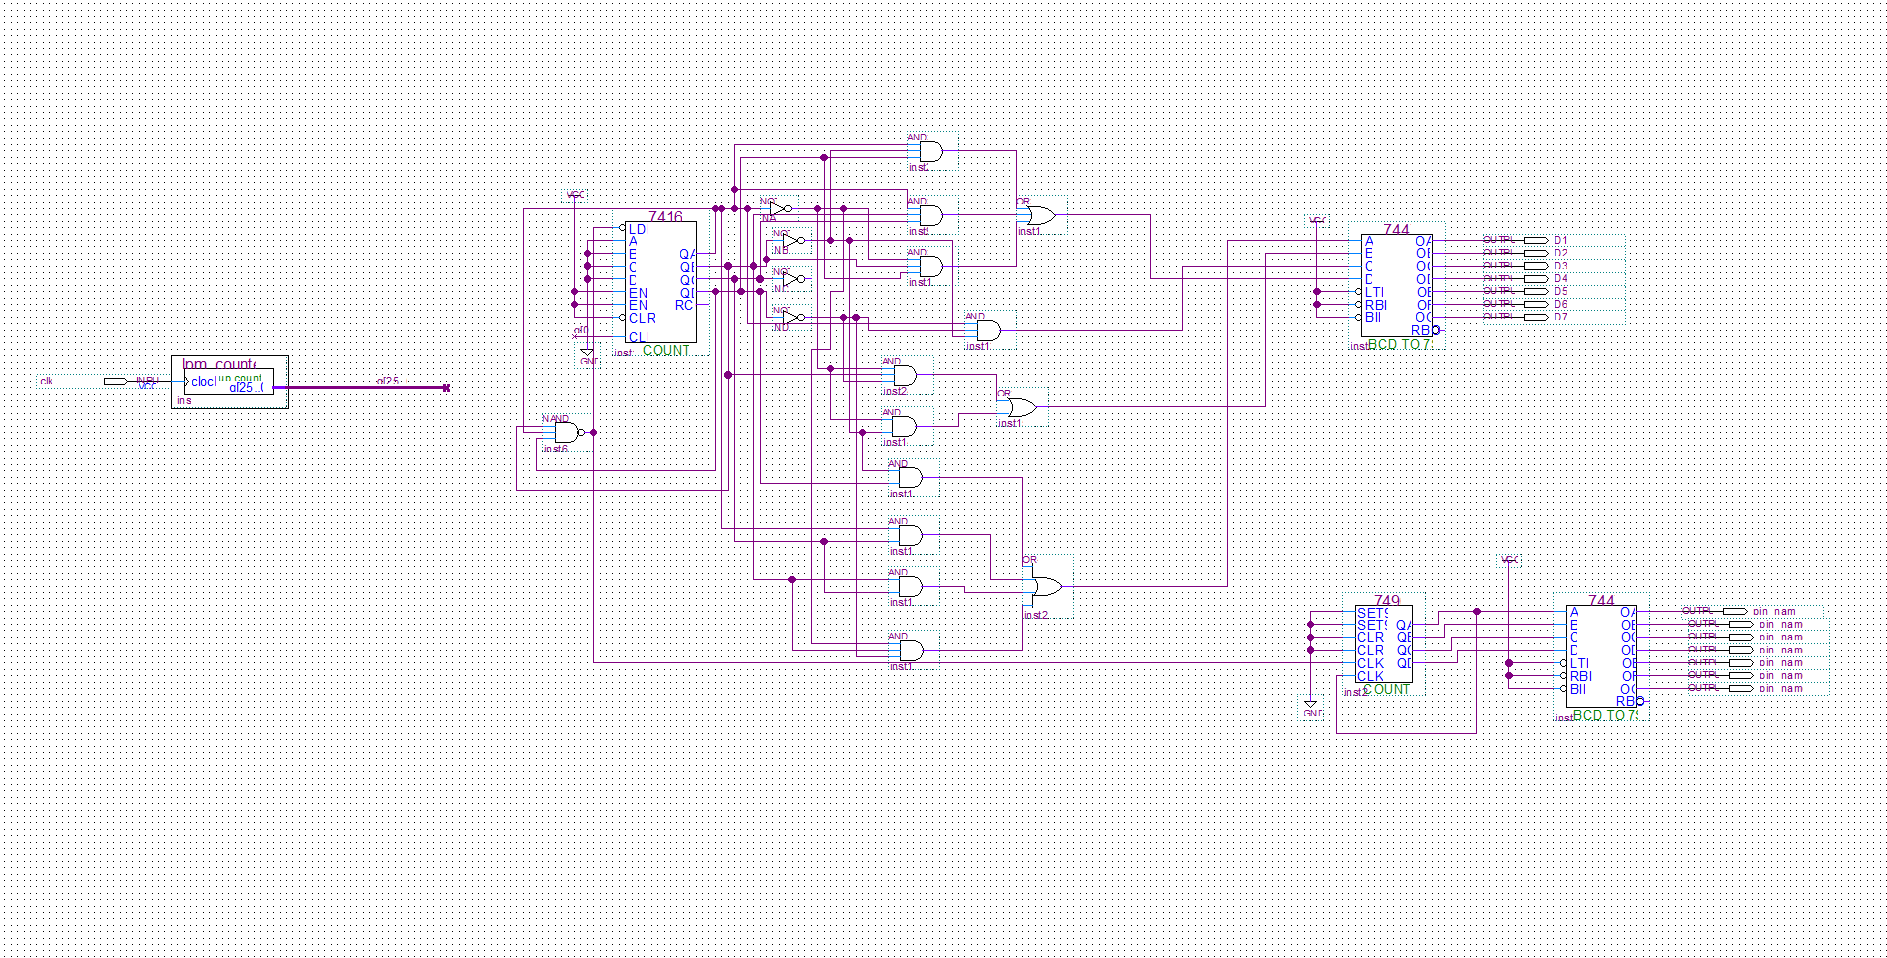
\includegraphics[width=0.95\textwidth]{仿真电路图.png}
    \caption{仿真电路图}
    \label{fig:circuit}
\end{figure}

\subsection{建立波形仿真文件}

选择 \textbf{File $\rightarrow$ New $\rightarrow$ Verification/Debugging $\rightarrow$ Vector Waveform File} 新建波形文件。通过 \textbf{Insert Node or Bus} 加入时钟、复位、计数器输出、7447 输入和七段输出信号。设置时钟信号周期，并在仿真开始时给复位端一个有效脉冲，使电路从第 0 轮开始显示。

运行仿真后，按顺序检查计数器输出和 7447 输入：轮次应依次变化，7447 输入应对应 \texttt{2,4,3,0,2,5,3,9,3,9,8,0}。再观察七段输出，确认每一轮对应的数码管显示数字正确。仿真结果如图~\ref{fig:wave} 所示。

\begin{figure}[H]
    \centering
    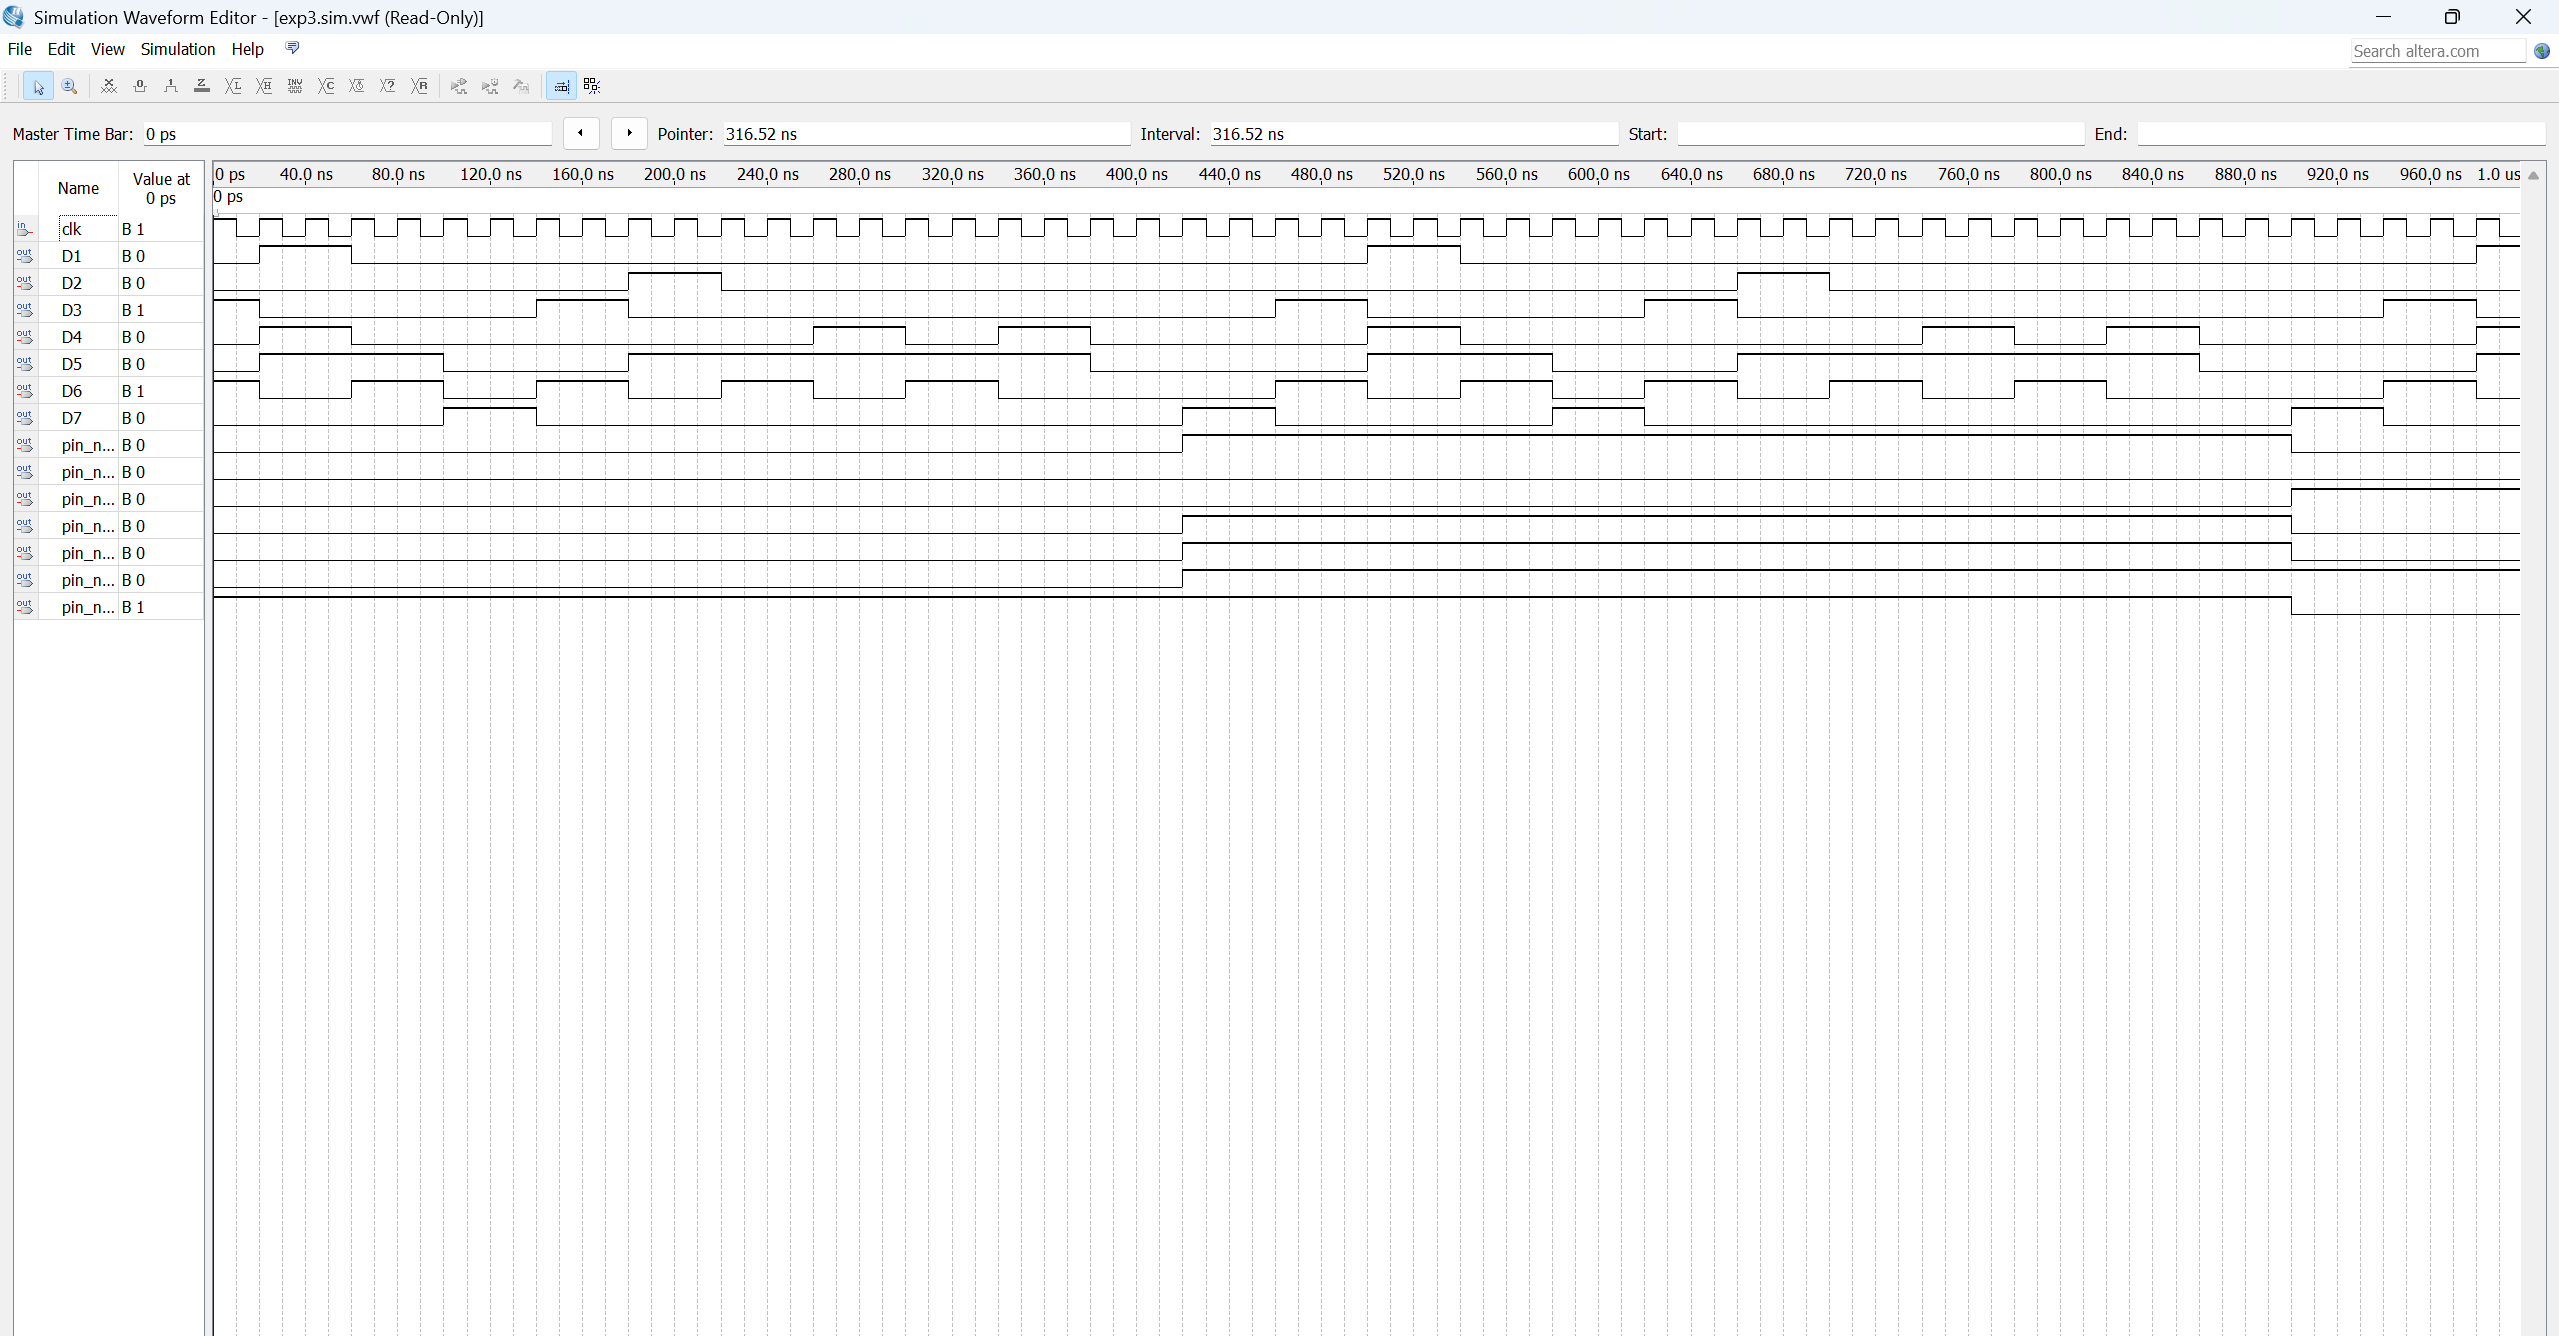
\includegraphics[width=\textwidth]{仿真波形图.png}
    \caption{仿真波形图}
    \label{fig:wave}
\end{figure}

\subsection{下载到 FPGA 验证}

仿真确认无误后，打开 Pin Planner，将时钟、复位和七段数码管输出分配到 DE0 开发板对应引脚。引脚分配完成后重新编译工程。随后连接 USB-Blaster，打开 Programmer，选择 JTAG 模式，加载生成的 \texttt{.sof} 文件并点击 \textbf{Start} 下载。

下载完成后，在开发板上观察 7 段数码管显示。按时钟输入变化时，数码管应按照 \texttt{243025393980} 的顺序循环显示。若显示顺序不对，返回检查计数器复位和序列选择逻辑；若数字笔段不对，返回检查 7447 输出与数码管段选引脚的对应关系。

\section{实验过程中的问题}

\begin{enumerate}
    \item 在设计显示电路时，需要区分 BCD 数字编码和七段数码管段选信号。若将二者直接混用，仿真中可能出现数字状态正确但数码管显示错误的问题，因此应先确定数字编码，再统一进行七段译码。
    \item 七段数码管存在高电平有效和低电平有效两种连接方式。仿真和实际下载验证时，应根据器件连接方式判断是否需要对段选信号取反，避免显示结果与预期数字相反或部分笔段异常点亮。
    \item 本实验目录中未提供 Verilog 源码或 Quartus 工程文件，因此报告主要依据实验说明和现有仿真截图整理，不额外列出代码清单。
\end{enumerate}

\section{心得体会}

\begin{enumerate}
    \item 通过本次实验，我进一步理解了时序逻辑电路和组合译码电路的配合方式。计数器负责产生状态，组合逻辑负责根据状态选择显示数字，七段译码器则把抽象数字转换为具体显示信号。
    \item 本次实验说明，数码管显示电路的关键不仅是写出数字序列，还要正确处理状态循环、编码转换和有效电平。通过观察仿真波形，可以较直观地检查显示顺序和段选输出是否符合设计要求。
\end{enumerate}

\end{document}
